
\subsection*{Sensor theory}
Sensor fusion can be observed everywhere e.g., living animals uses all of its senses to survive daily, an animal cannot hunt using its eyes only, it has to combine its sense of smell, eyes, and hearing to hunt the prey\cite{animal}. Sensor fusion theory is not only found in the living species it is found in cars, planes, computers and so on, this to enhance performance and accuracy. In this project, a sensor fusion will be designed to enhance the accuracy of the dinghy's position and velocity. The fusion will be a global positioning system,  \gls{gps} and an \gls{ins}. The \gls{ins} uses a low priced \gls{imu}.\\ 
The \gls{gps}'s accuracy is not uniform since there might be building reflections, atmospherics delays or clock bias errors \cite{boken}. Using the only information provided by a \gls{sins} is not sufficient either since the \gls{imu} sensor will drift after time, but using the information provided by the \gls{ins} for short time intervals will give more accurate results.  

\subsection{Inertial Navigation System}
In navigation there exist different techniques on how to navigate using an \gls{imu}, a typical technique is using a \gls{sins}. A \gls{sins} consists of an \gls{imu} which is mounted on the dinghy so it measures the acceleration and rotational rate that the dinghy encounters.
The concepts of inertial navigation are to determine the position and velocity of the dinghy from a known starting point, using only measurements from the \gls{imu}. The \gls{imu}, in this case, consists of a three-axis gyroscope, a three-axis accelerometer, and a three-axis magnetometer. \\
Measurement from the gyroscope is to determine the angular motion of the dinghy, from that its heading relative to a reference frame can be derived.
By measuring specific forces acting on the dinghy using the accelerometer, then resolve the specific force measurements into the reference frame using the knowledge derived from the information provided by the gyroscope. 
The resolved specific force measurements are integrated to obtain its velocity and position. \cite{non-linear} 


\subsection{Sensor fusion}
A popular filter to use when applying sensor fusion is to use a Kalman filter. The Kalman Filter is a recursive filtering method for discrete data, the algorithm was developed by a Hungarian mathematician Rudolf (Rudi) Emil Kalman in 1960 \cite{boken}. It's popular to use due to its efficiency when calculating predictions. \cite{kf eff}

\subsection{Navigation Frames}
Navigation algorithm involves various coordinate frames and therefore transformation between frames is a must. In this case, four different frames is used.\\

The Inertial frame denoted $i$-frame for future notation is defined such that its origin is at the center of Earth and its axes $X_i$, $Y_i$ and $Z_i$ is non-rotating with respect to the stars. $Z_i$ is coincident with the Earth's polar axis, i.e. North.\\

The Earth navigation frame denoted $e$-frame for future notation is fixed with respect to Earth and has its origin at the center of the Earth. The frame is defined as $X_e$, $Y_e$ and $Z_e$, with $Z_e$ along Earth's polar axis. Axis $X_e$ and $Y_e$ lies along the intersection of the plane of the Greenwich meridian with the Earth's equatorial plane. The $e$-frame rotates at a constant rate with respect to the $i$-frame and is denoted $\omega_e$.\\

The Navigation frame denoted $n$-frame for future notation is a local frame and has its origin located in the navigation system, in this case, point P, see Fig. \ref{WGS}, and its axes aligned with the directions of north, east and down, denoted NED. The turn rate of the navigation frame with respect to Earth's fixed frame, $\omega_{en}^n$, is directed by the motion of point P with respect to the Earth and is referred to the transport rate.   

\begin{figure}[H]
\centering
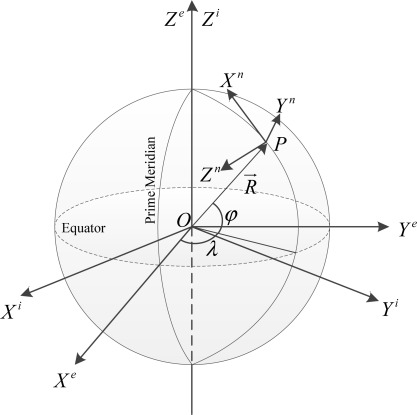
\includegraphics[width=0.3\textwidth]{Figures/WGS-coordinates.png}
\caption{Inertial, Earth and Navigation frame.}
\label{WGS}
\end{figure}

The Body frame denoted $b$-frame is the sensitive axes of the \gls{imu}'s sensors, which are made to coincide with the axes of the moving body in which the \gls{imu} is mounted in. The body, in this case, is referred to the dinghy, see Fig. \ref{Fig:body_frame}.

\begin{figure}[H]
\centering
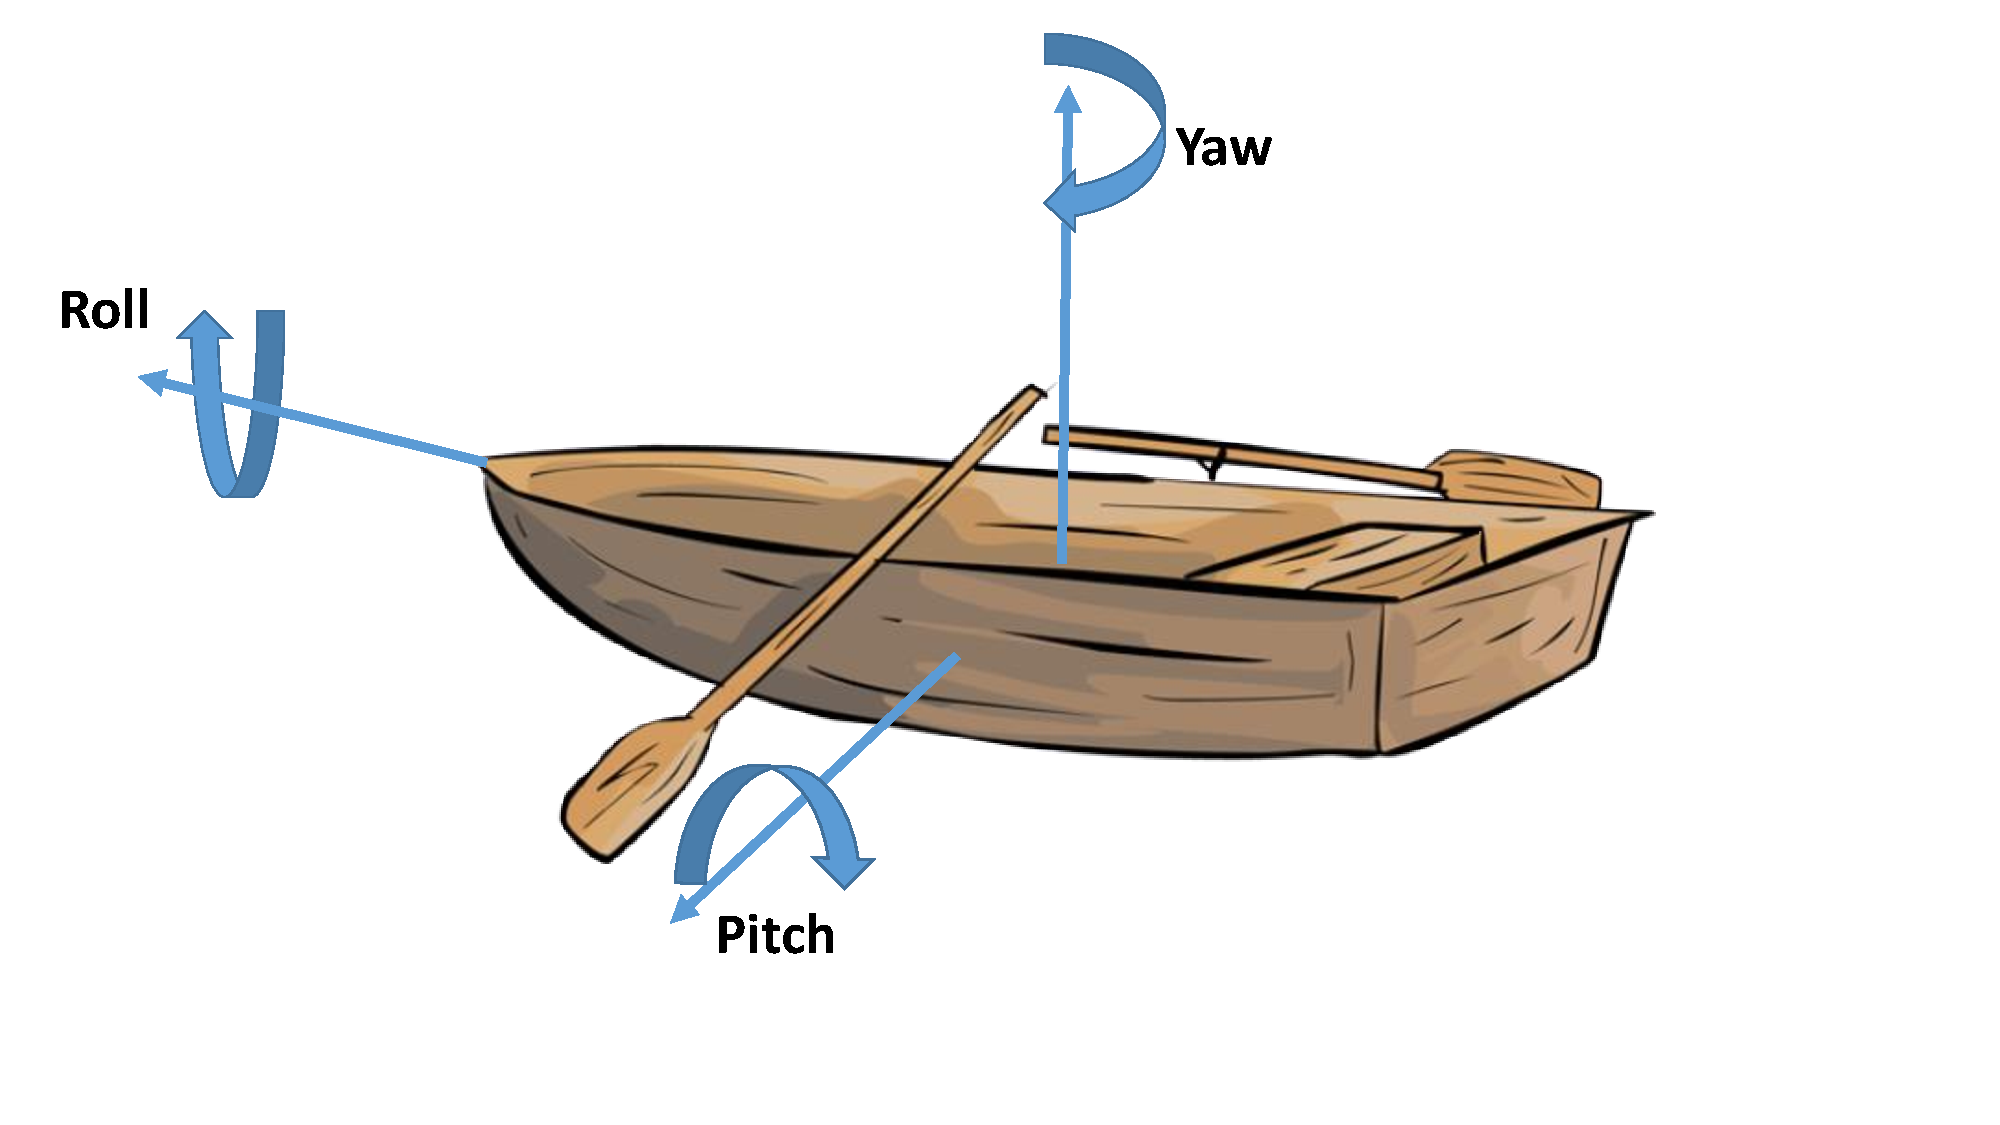
\includegraphics[width=0.5\textwidth]{Figures/Euler_angle.pdf}
\caption{Body frame}
\label{Fig:body_frame}
\end{figure}
\begin{itemize}
\item Yaw $(\psi)$: Is an imaginary line running vertically through the ship and through its center of gravity. A yaw motion is a side-to-side movement of the bow and stern of the dinghy \cite{SNAME}.
\item Pitch $(\theta)$: Is an imaginary line running horizontally across the ship and through the center of gravity. A pitch motion is an up-or-down movement of the bow and stern of the dinghy \cite{SNAME}.
\item Roll $(\phi)$: Is an imaginary line running horizontally through the length of the ship, through its center of gravity, and parallel to the waterline. A roll motion is a side-to-side or port-starboard tilting motion of the superstructure around this axis \cite{SNAME}.
\end{itemize}

\subsection{Transformation Between Frames}
Referring to Fig. \ref{WGS} it can be observed that its possible to align the $n$-frame with the $e$-frame, this is done by rotating the $n$-frame by ($\lambda-90$)-degrees around its $X$-axis (east-direction) and ($-\phi-90$)-degrees about its $Z$-axis, (downward direction) \cite{nonlinear}. Where $\lambda$ and $\varphi$ is the latitude and longitude, respectively. Then the transformation between the two frames can be done using the \gls{dcm}, which is defined as \cite{nonlinear}.
\begin{equation}
C_n^e=R_z(-\lambda-90)R_x(\varphi-90)
\label{Cosine_1}
\end{equation}
Where $C_n^e$ should be interpreted as moving from $n$-frame to $e$-frame, $R_x$ and $R_z$ are the rotation matrices around its axis, respectively. Expanding Eq. \eqref{Cosine_1} 
\begin{align}
C_n^e &=
\begin{bmatrix}
cos(-\lambda-90) & sin(-\lambda-90) & 0\\
-sin(-\lambda-90) & cos(-\lambda-90) & 0\\
0 & 0 & 1
\end{bmatrix}
\begin{bmatrix}
1 & 0 & 0\\
0 & cos(\varphi-90) & sin(\varphi-90) \\
0 & -sin(\varphi-90) & con(\varphi-90) \\
\end{bmatrix}\\
C_n^e &=
\begin{bmatrix}
-sin(\lambda) & -cos(\lambda) & 0\\
cos(\lambda) & -sin(\lambda) & 0\\
0 & 0 & 1
\end{bmatrix}
\begin{bmatrix}
1 & 0 & 0\\
0 & sin(\varphi) & -cos(\varphi) \\
0 & sin(\varphi) & sin(\varphi) \\
\end{bmatrix}\\
C_n^e &=
\begin{bmatrix}
-sin(\lambda) & -sin(\varphi)cos(\lambda) & cos(\varphi)cos(\lambda) \\
cos(\lambda) & -sin(\varphi)sin(\lambda) &  cos(\varphi)sin(\lambda) \\
0 & cos(\varphi) & sin(\varphi) \\
\end{bmatrix}
\end{align}
Exploring the orthogonality its possible to transform from $e$-frame to $n$-frame by taking the inverse of the equation above, i.e.
\begin{equation}
(C_n^e)^{-1}=C_e^n
\label{Eq.Earth2Nav}
\end{equation}
Using Eq. \eqref{Eq.Earth2Nav} its now possible to move from $e$-frame to $n$-frame. \\


Transforming from $n$-frame to $b$-frame is done in the same way, i.e. using rotation matrices. The \gls{dcm}, moving from $b$-frame to $n$-frame is given by \cite{nonlinear}
\begin{equation}
C_b^n=R_z(-\psi)R_y(-\theta)R_x(-\phi),
\label{Body_rotation}
\end{equation}
where 
\begin{align}
R_z(-\psi) = &
\begin{bmatrix}
cos(\psi) & -sin(\psi) & 0\\
sin(\psi) & cos(\psi) & 0 \\
0 & 0 & 1
\end{bmatrix}\label{R_z} \\
R_y(-\theta) = &
\begin{bmatrix}
cos(\theta) & 0 & sin(\theta)\\
0 & 1 & 0 \\
-sin(\theta) & 0 & cos(\theta)
\end{bmatrix}\label{R_y} \\
R_x(-\phi) = &
\begin{bmatrix}
1 & 0 & 0\\
0 & cos(\phi) & -sin(\phi)\\
0 & sin(\phi) & cos(\phi)
\end{bmatrix}\label{R_x}
\end{align}
Solving Eq. \eqref{Body_rotation} with \eqref{R_z}, \eqref{R_y} and \eqref{R_x}
\begin{align}
C_b^n = &
\begin{bmatrix}
cos(\psi) & -sin(\psi) & 0\\
sin(\psi) & cos(\psi) & 0 \\
0 & 0 & 1
\end{bmatrix}
\begin{bmatrix}
cos(\theta) & 0 & sin(\theta)\\
0 & 1 & 0 \\
-sin(\theta) & 0 & cos(\theta)
\end{bmatrix}
\begin{bmatrix}
1 & 0 & 0\\
0 & cos(\phi) & -sin(\phi)\\
0 & sin(\phi) & cos(\phi)
\end{bmatrix}
\label{expand_Body_rotation} \\ \\
C_b^n  = & 
\begin{bmatrix}
cos(\theta)cos(\psi) & -cos(\phi)sin(\psi)+sin(\phi)sin(\theta)cos(\psi) &  sin(\phi)sin(\psi)+cos(\phi)sin(\theta)cos(\psi) \\
cos(\theta)sin(\psi) & cos(\phi)cos(\psi)+sin(\phi)sin(\theta)sin(\psi) & -sin(\phi)cos(\psi)+cos(\phi)sin(\theta)sin(\psi)\\
-sin(\theta) & sin(\phi)cos(\theta) & cos(\phi)cos(\theta) 
\end{bmatrix}.
\end{align}
Where $\psi$, $\theta$ and $\phi$ are the Euler angles as described earlier. Expressing the matrix above in a more compact form.
\begin{align}
C_b^n = &
\begin{bmatrix}
c_{11} && c_{12} && c_{13}\\
c_{21} && c_{22} && c_{23} \\
c_{31} && c_{32} && c_{33}
\end{bmatrix}
\label{Eq.C_b_n_compact}
\end{align}
The Euler angles is a transformation from one coordinate frame to another and is defined by three successive rotations about the different axis. Its possible to see the three angles as a set of mechanical gimbals. 
The problem with Euler angles is that when rotating about each axis, its possible to drive two of the three gimbals so they appear parallel to each other this implies that a degree of freedom is lost, this is called a gimbal-lock \cite{nonlinear}. To resolve this issue its possible to use quaternion attitude representation instead, as Euler angels the representation allows transformation between one coordinate frame to another, but the difference is that the transformation is done in a single rotation, instead of three about a vector defined in the reference frame. The \gls{dcm} using quaternion is defined such that\cite{nonlinear}.
\begin{align}
C_b^n & =
\begin{bmatrix}
(q_1^2 + q_2^2 - q_3^2-q^4) && 2(q_2q_3 - q_1q_4) && 2(q_2q_4 + q_1q_3) \\
2(q_2q_3 - q_1q_4) && (q_1^2 - q_2^2 + q_3^2-q^4) && 2(q_3q_4 - q_1q_2) \\
2(q_2q_4 - q_1q_3) && 2(q_3q_4 + q_1q_2) && (q_1^2 - q_2^2 - q_3^2+q^4)
\end{bmatrix}
\end{align}

Where $q_1$, $q_2$, $q_3$ and $q_4$ can be derived using the Euler angles from Eq. \eqref{Eq.C_b_n_compact}
\begin{align*}
q_1 =& \frac{1}{2}(1+c_{11} + c_{22} + c_{33})^{0.5} \\
q_2 =& \frac{1}{4q_1}(c_{32} - c_{23})\\
q_3 =& \frac{1}{4q_1}(c_{13} - c_{31})\\
q_4 =& \frac{1}{4q_1}(c_{21} - c_{12})\\
\end{align*}


The angular velocity of the $e$-frame with respect to the $i$-frame projected onto the $e$-frame is given as \cite{nonlinear}
\begin{equation}
\bar{\omega}_{ie}^e = 
\begin{bmatrix}
0 & 0 & \omega_e
\end{bmatrix}^T.
\end{equation}
Where $\omega_e$ is the angular velocity of the Earth and has a value of
$7.2921158 \times 10^{-5}$ $rad/s$ \cite{nonlinear}. Using the projection matrix Eq. \eqref{Cosine_1} its possible to project $\bar{\omega}_ {ie}^i$ onto the $n$-frame
\begin{align}
\bar{\omega}_{ie}^n=C_e^n\bar{\omega}_{ie}^e=
\begin{bmatrix}
\omega_e cos(\varphi) & 0 & -\omega_e sin(\varphi)
\end{bmatrix}^T.
\label{omega_ie}
\end{align}
$\bar{\omega}_{en}^n$ represents the turn rate of the $n$-frame with respect to the $e$-frame its called the transport rate and may be expressed as the rate of change of latitude and longitude as follows
\begin{align}
\bar{\omega}_{en}^n=
\begin{bmatrix}
\dot{\lambda}cos(\varphi) & -\dot{\varphi} & -\dot{\lambda}sin(\varphi)
\end{bmatrix}^T.
\label{omega_en}
\end{align}
Where $\dot{\lambda}=v_e/(R_N+h)cos(\varphi)$ and $\dot{\varphi}=v_n/(R_E+h)$ \cite{nonlinear}, here we assume the Earth to be an ellipsoid and that there are no variations in Earth's gravitation depending on where the user is on the ellipsoid. $R_N$ is the meridian radius of curvature and defined as $R_N=R_0(1-e^2)/(1-e^2sin^2\varphi)^{3/2}$ \cite{nonlinear}. $R_E$ is the transverse radius of curvature and defined as $R_E=R_0/(1-e^2sin^2\varphi)^{1/2}$. Where $R_0$ is the length of the semi-major axis and has a constant value of $6356752.3142$ m, $e$ is the major eccentricity of the ellipsoid and has a constant value of $0.081819$, $\varphi$ is the current latitude in radians, $v_N$ and $v_E$ is the velocity in north and east direction, respectively and $h$ is the height above the surface of the Earth. Then Rewriting Eq. \eqref{omega_en} with the new expressions.
\begin{align}
\bar{\omega}_{en}^n=
\begin{bmatrix}
v_e/(R_E+h) & -v_n/(R_N+h) & -v_e tan(\varphi)/(R_N+h)
\end{bmatrix}^T \label{omega_en_ny}
\end{align}
Now the turn rate of the $n$-frame with respect to $i$-frame, $\bar{\omega}_{in}^n$ can be obtained by adding Eq. \eqref{omega_ie} and \eqref{omega_en_ny} together.
\begin{align}
\bar{\omega}_{in}^n=
\begin{bmatrix}
\omega_e cos(\varphi) + v_e/(R_E+h) & v_n/(R_N+h) & -\omega_e sin(\varphi) + v_e tan(\varphi)/(R_N+h)
\end{bmatrix}^T
\label{Eq.omega_in}
\end{align}

\noindent Now Eq. \eqref{Eq.omega_in} is a function dependent both on velocity and position.

\subsection{Inertial Navigation Equation}
Describing the position of the dinghy in the $n$-frame is done by \cite{nonlinear}.
\begin{align}
\bar{r}^n=
\begin{bmatrix}
\varphi & \lambda & h
\end{bmatrix}^T.
\end{align}
Since velocity is described as the rate of change of its position with respect to a frame of reference and is a function of time, the velocities in the north, east and down can be expressed as.
\begin{align}
\begin{bmatrix}
v_N \\
v_E \\
v_D
\end{bmatrix}
=
\begin{bmatrix}
(R_E+h) & 0 & 0 \\
0 & (R_N+h)cos(\varphi) & 0\\
0 & 0 & -1
\end{bmatrix}
\begin{bmatrix}
\dot{\varphi}\\
\dot{\lambda}\\
\dot{h}
\end{bmatrix}
\label{Eq.v_n1}
\end{align}
Where $\dot{-}$ symbolizes the first derivative with respect to time. Thus, $\dot{\varphi}$, $\dot{\lambda}$ and $\dot{h}$ can be derived by rewriting Eq. \eqref{Eq.v_n1} as

\begin{align}
\begin{bmatrix}
\dot{\varphi}\\
\dot{\lambda}\\
\dot{h}
\end{bmatrix}
=
\underbrace{\begin{bmatrix}
\frac{1}{(R_E+h)} & 0 & 0 \\
0 & \frac{1}{(R_N+h)cos(\varphi)} & 0\\
0 & 0 & -1
\end{bmatrix}}_{D^{-1}}
\begin{bmatrix}
v_N \\
v_E \\
v_D
\end{bmatrix}
\label{Eq.v_n}
\end{align}

\noindent Thus the dynamics describing the system can be expressed as \cite{nonlinear}.

\begin{align}
\dot{\bar{r}}_n = & D^{-1}v_n
\label{Eq.r_n_t}\\
\dot{\bar{v}}_n = & C_b^n \bar{f}^b-(2\omega_{ie}^n+\omega_{en}^n) \times \bar{v}_n +\bar{g}^n
\label{Eq.v_n_t}\\
\dot{C}_b^n = & C_b^n(\Omega_{ib}^b - \Omega_{in}^b)
\label{Eq.C_b_n_t}
\end{align}
Where $\bar{f}^b$ is the specific force vector defined as the difference between the true acceleration in
space and the acceleration due to gravity and $\bar{g}^n$ is the gravity vector. Where $\Omega$ is the skew matrix of $\omega$, more precise $\Omega_{ib}^b$ the skew-matrix of the outputs of the strapdown gyroscopes and $\Omega_{in}^n$ is the skew-matrix of Eq. \eqref{Eq.omega_in}. Skew-matrix is defined as the cross product between the vectors.


\subsection{INS mechanization}
Since the INS has to work in discrete time domain, Eq. \eqref{Eq.r_n_t}, \eqref{Eq.v_n_t} and \eqref{Eq.C_b_n_t} has to be discretized. The sampling time should be seen as a changing variable since it may not be constant instead it will fluctuate around $100Hz$, this means that $\Delta t_k = \Delta k_{k-1} - t_{k}$, this to improve the accuracy. The discrete dynamics are \cite{non-linear}, Using Eq. \eqref{Eq.r_n_t},\eqref{Eq.v_n_t} and \eqref{Eq.C_b_n_t}.


\begin{align}
\bar{r}_{k+1}^n = & \bar{r}_k + 0.5D^{-1}(\bar{v}_k^n + \bar{v}_{k+1}^n)\Delta t
\label{Eq.r_n_d}\\
v_{k+1}^n= & \bar{v}_k + \Delta \bar{v}_{k+1}^n
\label{Eq.v_n_d}\\
\dot{C}_b^n = & C_b^n(\Omega_{ib}^b - \Omega_{in}^b)\Delta t
\label{Eq.C_b_n_d}
\end{align}
where 
\begin{equation}
\Delta \bar{v}_{k+1}^n = \Delta \bar{v}_f^n - (2\omega_{ie}^n+\omega_{en}^n) \times \bar{v}_n \Delta t +\bar{\gamma}\Delta t
\end{equation}
where $\gamma = [0 \quad 0 \quad 9.8123]$.\\ \\
The Navigation frame Inertial Navigation System can now be seen in Fig. \ref{Fig:body_frame}, Where its possible to examine all the steps which were derived earlier, from the \gls{imu} to the output.
\begin{figure}[H]
\centering
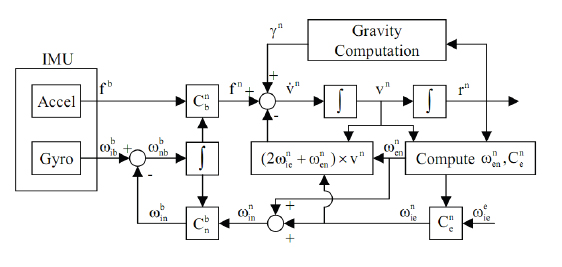
\includegraphics[width=0.7\textwidth]{Figures/ins_2}
\caption{The Inertial Navigation Frame}
\label{Fig:body_frame}
\end{figure}
\section{Implementation of Sensor Fusion Using a Kalman Filter.}
\subsection*{Perturbation Analysis}
Since the differential equations describing velocity, position, and the attitude, \gls{dcm} are non-linear, utilize a perturbation series to minimize the errors \cite{pertubation}.
\begin{equation}
\hat{r}^n =r^n+\delta r^n
\label{Eq.per_r}
\end{equation}
\begin{equation}
\hat{v}^n =v^n+\delta v^n
\label{Eq.per_v}
\end{equation}
\begin{equation}
\hat{C}_b^n = (I-E^n)C_b^n
\label{Eq.per_c}
\end{equation}
Where $E^n$ is the skew matrix and given as.
\begin{align}
\begin{bmatrix} 
0 && -e_D && e_E \\
e_D && 0 && -e_N \\
-e_E && e_N && 0
\end{bmatrix}
\end{align}
Where $\hat{}$ is the computed values, $\delta$ and $e_{NED}$ are the errors in North, East and upward direction, respectively.

\subsubsection{Error Dynamics Position}
Perturbing \eqref{Eq.per_r}, the linearized position is obtained since the position dynamics is a function of both position and velocity, the position error dynamics is obtained as
\begin{equation}
\delta \dot{\bar{r}}^n = F_{rr}\delta \bar{r}^n + F_{rv}\delta \bar{v}^n.
\end{equation}

\noindent Where
\begin{align}
F_{rr} &=
\begin{bmatrix}
0 && 0 && \frac{-v_N}{(M+h)^2}\\
\frac{v_E sin(\varphi)}{(N+h)cos^2(\varphi)} && 0 && \frac{-v_E}{(N+h)^2cos(\varphi)} \\
0 && 0 && 0
\end{bmatrix}
\label{Eq.Frr}
\end{align}
and
\begin{align}
F_{rv} &=
\begin{bmatrix}
\frac{1}{(M+h)} && 0 && 0\\
0 && \frac{1}{(N+h)cos(\varphi)} && 0 \\
0 && 0 && -1
\end{bmatrix}.
\label{Eq.Frv}
\end{align}
\subsubsection{Error Dynamics Velocity}
The same is used when deriving the perturbation for the velocity, Eq. \eqref{Eq.per_v}, here, velocity is described by forces and gravity acting on the dinghy. Using Eq. \eqref{Eq.v_n_t}, and perturbation Eq. \eqref{Eq.per_v}, the following is obtained \cite{nonlinear}.
\begin{equation}
\delta \dot{\bar{v}}^n = \bar{v}_n \times \underbrace{(2\delta \bar{\omega}_{ie}^n+ \delta \bar{\omega}_{en}^n)}_{I}+\delta \bar{g}^n -\underbrace{(2\bar{\omega}_{ie}^n + \bar{\omega}_{en}^n)}_{II}\times \delta \bar{v}^n + (\bar{f}^n\times) e^n +C_b^n\delta \bar{f}^n
\label{Eq.delta_v}
\end{equation}
where $II$ is expressed as follow, using Eq. \eqref{Eq.omega_in}.
\begin{align}
2\bar{\omega}_{ie}^n + \bar{\omega}_{en}^n = 
\begin{bmatrix}
2\omega_e cos(\varphi) + \frac{v_E}{(N+h)} \\
\frac{-v_N}{(M+h)} \\
-2\omega_e sin(\varphi) - \frac{v_E tan(\varphi)}{(N+h)}
\end{bmatrix}.
\label{Eq.II}
\end{align}
Now perturbing $I$ with $II$, using Eq. \eqref{omega_en} and \eqref{Eq.omega_in}, the following is obtained.
\begin{align}
2\delta \bar{\omega}_{ie}^n+ \delta \bar{\omega}_{en}^n =
\delta \Omega_r\delta \bar{r}^n + \delta\Omega_r\delta\bar{v}^n
\end{align}
where
\begin{align}
\delta\Omega_r = 
\begin{bmatrix}
-2 \omega_e sin(\varphi) && 0 && \frac{-v_E}{(N+h)^2}\\
0 && 0 && \frac{v_N}{(M+h)^2}\\
2 \omega_e cos(\varphi)-\frac{v_E}{(N+h)cos^2(\varphi)} && 0 && \frac{v_E tan(\varphi)}{(N+h)^2}
\end{bmatrix}
\label{Eq.Omega_r}
\end{align}
and
\begin{align}
\delta\Omega_v = 
\begin{bmatrix}
0 &&  \frac{-1}{(N+h)} && 0\\
\frac{-1}{(M+h)} && 0 && 0\\
0 && \frac{-tan(\varphi)}{(N+h)} && \frac{v_E tan(\varphi)}{(N+h)^2}
\end{bmatrix}
\label{Eq.Omega_v}
\end{align}
Then calculating the first term on the left side of Eq. \eqref{Eq.delta_v}, using Eq. \eqref{Eq.Omega_r} and \eqref{Eq.Omega_v}
\begin{align}
\bar{v}^n\times(2\delta \bar{\omega}_{ie}^n+\delta \bar{\omega}_{en}^n) = 
\bar{v}^n \times \delta\Omega_r\delta\bar{r}^n +\bar{v}^n\times\delta\Omega_v\delta\bar{v}^n
\end{align}
Then expressing Eq. \eqref{Eq.delta_v} as
\begin{equation}
\delta\bar{v}^n = F_{vr}\delta\bar{r}^n + F_{vv}\delta\bar{v}^n + (\bar{f}^n	\times)\bar{e}^n + C_n^b\delta \bar{f}^b
\end{equation}
Expressing $F_{vr}$ and $F_{vv}$ in matrix notation
\begin{align}
F_{vr} = 
\begin{bmatrix}
-2v_E\omega_e cos(\varphi)-\frac{v_E^2}{(N+h)cos^2(\varphi)} && 0 && \frac{-v_N v_D}{(M+h)^2} + \frac{v_E^2 tan(\varphi)}{(N+h)^2} \\
2\omega_e(v_N cos(\varphi)-v_D sin(\varphi)) + \frac{v_Ev_N}{(N+h)cos^2(\varphi)} && 0 && \frac{-v_E v_D}{(N+h)^2} - \frac{v_Nv_E tan(\varphi)}{(N+h)^2} \\
2v_E\omega_e sin(\varphi) && 0 && \frac{v_E^2}{(N+h)^2} + \frac{v_N^2}{(M+h)^2} - \frac{2\gamma}{R+h}
\end{bmatrix}
\label{Eq.Fvr}
\end{align}
and
\begin{align}
F_{vv} = 
\begin{bmatrix}
\frac{v_D}{(M+h)} && -2\omega_e sin(\varphi) -2\frac{v_Etan(\varphi)}{(N+h)} && \frac{v_N}{(M+h)} \\
2\omega_e sin(\varphi) +\frac{v_E tan(\varphi)}{(N+h)} && \frac{v_D + v_N tan(\varphi)}{(N+h)} && 2\omega_e cos(\varphi)+ \frac{v_E}{(N+h)} \\
-2\frac{v_N}{(M+h)} && -2\omega_e cos(\varphi) -2\frac{v_E}{(N+h)} && 0
\end{bmatrix}
\label{Eq.Fvv}
\end{align}
\subsubsection{Error Dynamics Attitude}
The output from the \gls{ins} can be expressed using Eq. \eqref{Eq.C_b_n_t}.
\begin{equation}
\hat{\dot{C}}_b^n = \hat{C}_b^n(\hat{\Omega}_{ib}^b - \hat{\Omega}_{in}^b)
\end{equation}
Then relate the above equation with Eq. \eqref{Eq.per_c}
\begin{equation}
-\dot{E}^nC_b^n = (I_E^n)C_b^n(\delta\Omega_{ib}^b-\delta\Omega_{in}^b)
\end{equation}
Expressing $\dot{E}^n$ by is self in left-hand side, the equation above can be expressed as
\begin{equation}
\dot{E}^n = -C_b^n(\delta\Omega_{ib}^b-\delta\Omega_{in}^b)
\end{equation}
or in vector form
\begin{equation}
\dot{\bar{e}}^n = -C_b^n(\delta\omega_{ib}^b-\delta\omega_{in}^b).
\label{Eq.error_vec}
\end{equation}

Since we want to express the equation above in its error equation $\delta \bar{\omega}_{in}^b$, the following change can be done $\hat{\bar{\omega}}_{in}^b = \hat{C}_n^b\hat{\bar{\omega}}_{in}^n$ This can be expanded into
\begin{equation}
\bar{\omega}_{in}^b + \delta \bar{\omega}_{in}^b = C_b^n(I+E^n)(\bar{\omega}_{in}^n+\delta\bar{\omega}_{in}^n).
\end{equation}
Using vector notation for the skew matrix, the equation above can be written as
\begin{equation}
\delta\bar{\omega}_{in}^b = C_n^b [\delta\bar{\omega}_{in}^n + (e^n\times)\bar{\omega}_{in}^n].
\label{Eq.del_omega}
\end{equation}
Substituting Eq. \eqref{Eq.del_omega} into Eq. \eqref{Eq.error_vec}, the following is obtained

\begin{equation}
\dot{\bar{e}}^n = \delta\bar{\omega}_{in}^n -(\bar{\omega}_{in}^n \times )\bar{e}^n - C_b^n\delta \bar{\omega}_{ib}^b 
\label{Eq.err_final}
\end{equation}
Then expressing the first term on the right-hand side into the position and velocity error terms explicitly, using Eq. \eqref{Eq.v_n} and \eqref{Eq.II}. The error attitude dynamics is then obtained and written as
\begin{equation}
\dot{\bar{e}}^n = F_{er}\delta \bar{r}^n + F_{ev}\delta \bar{v}^n - (\bar{\omega}_{in}^n \times)\bar{e}^n - C_b^n\delta\bar{\omega}_{ib}^b.
\end{equation}
Where $F_{er}$ and $F_{ev}$ is	
\begin{align} = 
F_{er} =
\begin{bmatrix}
-\omega_e sin(\varphi) && 0 && \frac{-v_E}{(N+h)^2}\\
0 && 0 && \frac{v_N}{(M+h)^2} \\
\omega_e cos(\varphi) - \frac{v_E}{(N+h)cos^2(\varphi)} && 0 && \frac{v_E tan(\varphi)}{(N+h)^2}
\end{bmatrix}
\label{Eq.Fer}
\end{align}

\begin{align} = 
F_{ev} =
\begin{bmatrix}
0 && \frac{1}{(N+h)} && 0\\
\frac{-1}{(M+h)} && 0 && 0\\
0 && \frac{-tan(\varphi)}{(N+h)} && 0
\end{bmatrix}.
\label{Eq.Fev}
\end{align}

\subsection{Implementing the Fusion Kalman Filter}
This system uses a feedback method to control the drift errors in the \gls{imu}, the model can be seen in Fig. \ref{Fig:Feedback}.
\begin{figure}[H]
\centering
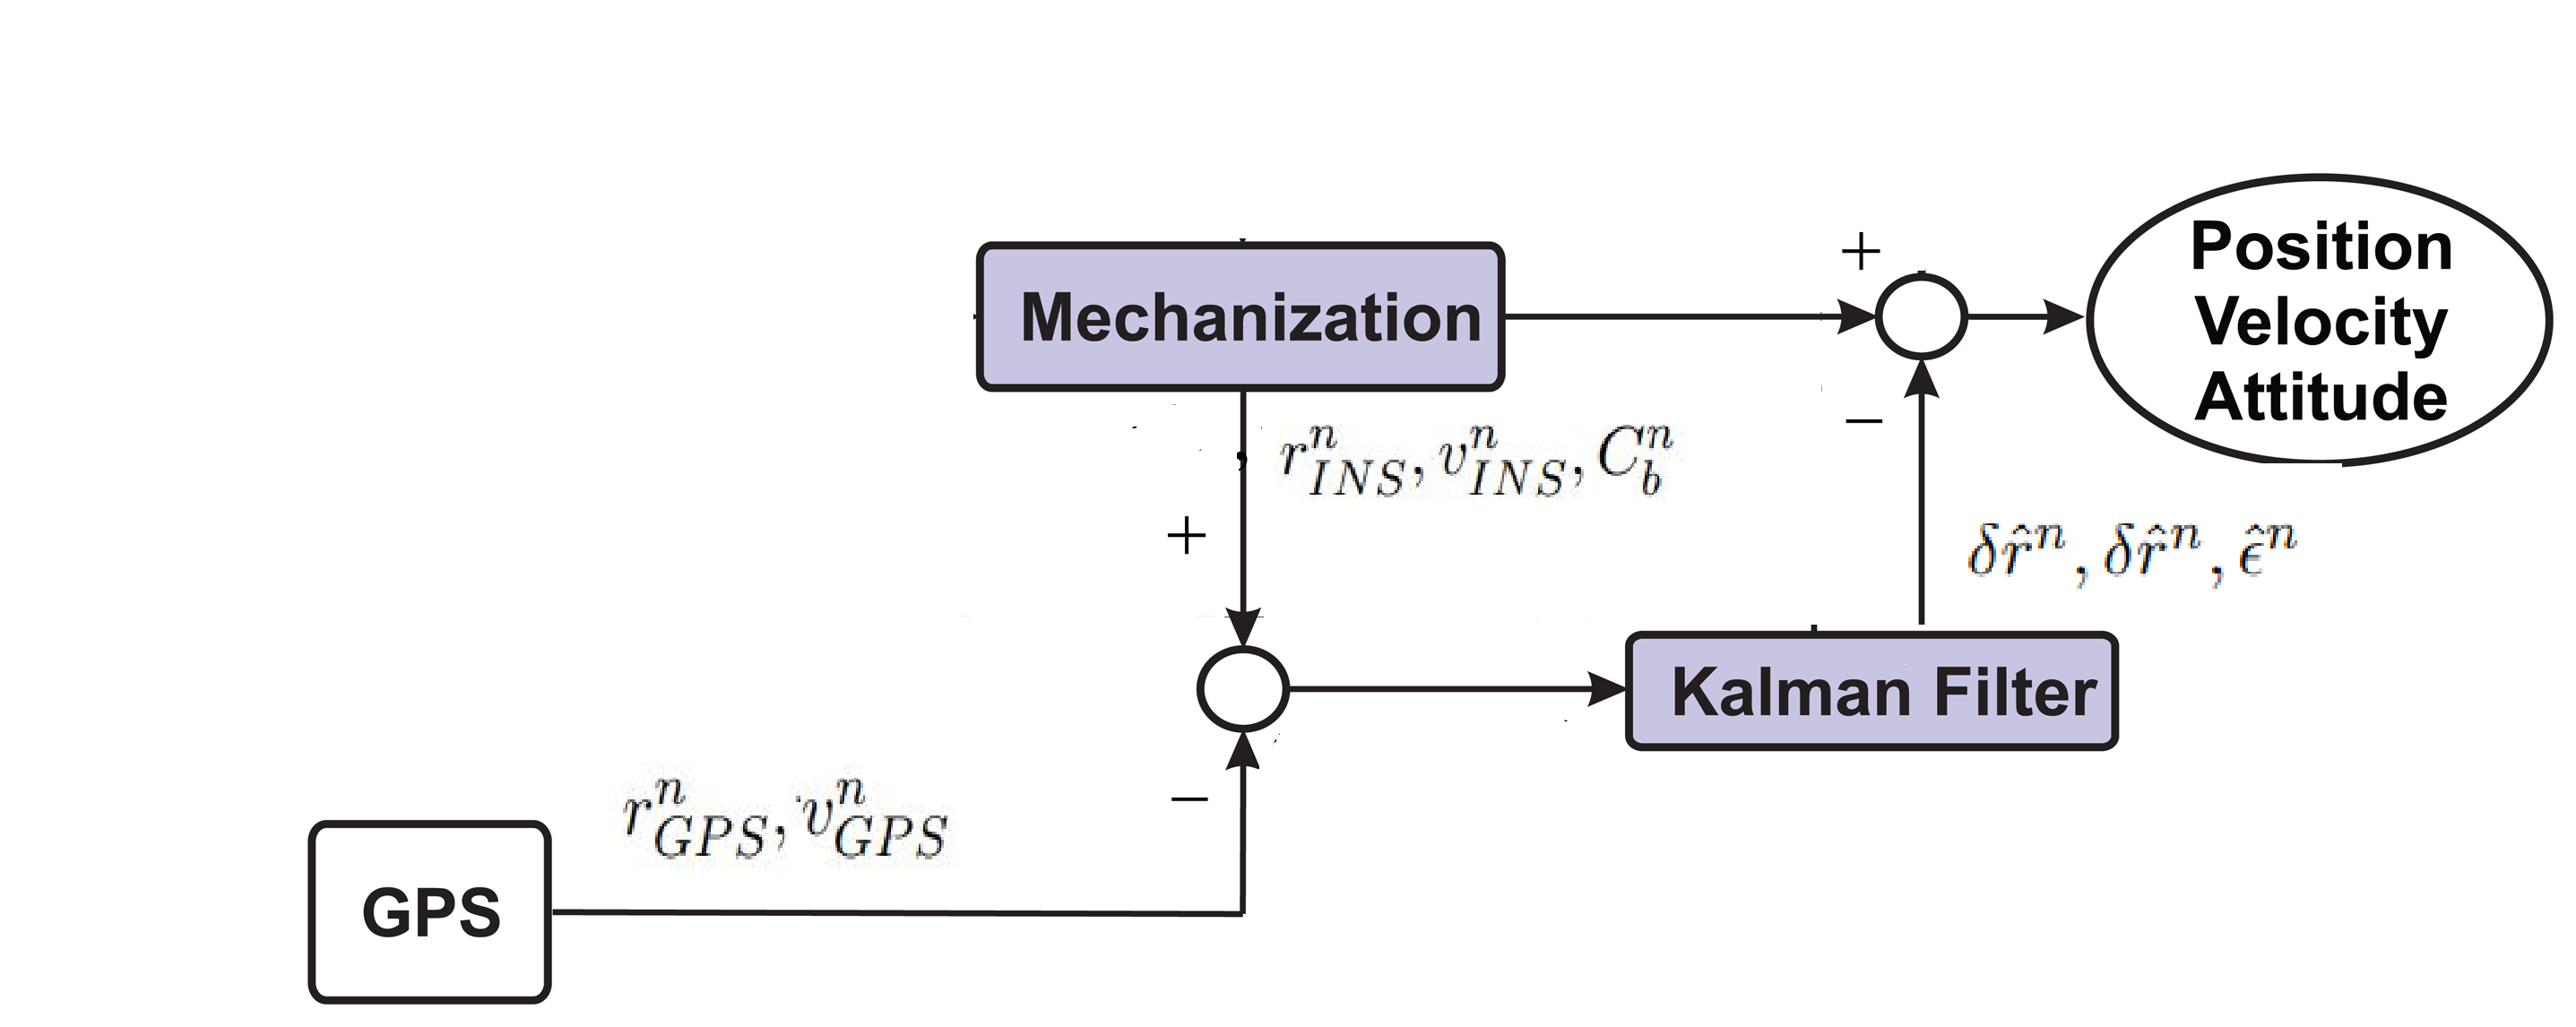
\includegraphics[width=0.7\textwidth]{Figures/feed-back.png}
\caption{The feedback-method which is used in the system.}
\label{Fig:Feedback}
\end{figure}
Implementing a continuous Kalman Filter using integration between Inertial Navigation System and a Global Positioning System.
\begin{align}
\hat{\bar{x}} = F \bar{x} + G \bar{u}
\label{eq.state_1}
\end{align}
Where $F$ is describing the dynamics of the system, $\bar{x}$ is the state vector, $G$ is the design matrix, $\bar{u}$ is the input matrix, i.e. forces acting on the dinghy recorded by the \gls{imu} and $\hat{\bar{x}}$ is the estimated state vector. \\

Where $F$ is a $9\times 9$ matrix and contain Eq. \eqref{Eq.Frr}, \eqref{Eq.Frv}, \eqref{Eq.Fvr}, \eqref{Eq.Fvv}, \eqref{Eq.Fer}, \eqref{Eq.Fev}, \eqref{Eq.omega_in}, and $\bar{x}$ is a $9 \times 1$ is given by
\begin{align}
F=
\begin{bmatrix}
F_{rr} & F_{rv} & 0 &\\
F_{vr} & F_{vv} & (\bar{f}^n \times)\\
F_{er} & F_{ev} & -(\bar{\omega}_{in}^n\times)
\end{bmatrix},
\qquad
\bar{x}=
\begin{bmatrix}
\delta\bar{r}^n \\
\delta\bar{v}^n\\
\delta\bar{e}^n
\end{bmatrix}
\end{align}
$G$ is a $6\times6$ matrix and $\bar{u}$ is a $6 \times 1$ vector and is defined as.
\begin{align}
G=
\begin{bmatrix}
-C_b^n & 0 \\
0 & C_b^n
\end{bmatrix},
\qquad
\bar{u}=
\begin{bmatrix}
\delta \bar{\omega}_{ib}^b \\
\delta \bar{f}^b 
\end{bmatrix}
\end{align}
The elements of $\bar{u}$ is assumed to be white noise with zero mean, thus
\begin{align}
Q=diag
\begin{bmatrix}
\sigma^2_{ax} & \sigma^2_{ay} & \sigma^2_{az} & \sigma^2_{gx} & \sigma^2_{gy} & \sigma^2_{gz}
\end{bmatrix}^T
\label{Eq.Q}
\end{align}
where $\sigma^2_{a(x,y,z)}$ and $\sigma^2_{g(x,y,z)}$ is the variance for the accelerometer and gyroscope in every direction, respectively.\\
	
Since a computer does not use continuous time domain the equation has to be transformed into discrete domain. The state equation will then be expressed as
\begin{equation}
\hat{\bar{x}}_{k+1} = \Phi_k \bar{x}_k +  \bar{w}_k	
\label{Eq.discrete}
\end{equation}
Here $\Phi_k$ is the state transition matrix in discrete time domain, in order to obtain a discrete state transition matrix the inverse Laplace transform is performed on the continuous state transition matrix, i.e.
\begin{equation}
\Phi_k = \mathcal{L}^{-1}\big[(SI-F)^{-1}\big]
\label{Eq.Phik}
\end{equation}
Since the sample interval, $\Delta t$ is very small in this case Eq. \eqref{Eq.Phik} can be approximated using Taylor approximation 
\begin{equation}
\Phi_k = e^{F\Delta t} \approx I + F \Delta t 
\label{Eq.Final_Phik}.
\end{equation}
From Eq. \eqref{Eq.discrete}, $\hat{w}_k$ is the driven response $t_{k+1}$ due to the input white noise. White noise is uncorrelated between sample periods, i.e the noise between $t_k$ and $t_{k+1}$ is uncorrelated \cite{signal_process}. Then the covariance matrix which is associated with $\bar{w}_k$ is \cite{signal_process}

\begin{align}
\mathbb{E}[\bar{w_i}\bar{w}_j^T] =
\begin{cases}
  Q_k &\quad i=j\\    
  0 &\quad i\neq j   
\end{cases}
\end{align}

and $Q_k$ can then be approximated using a first order of the discrete transition matrix \cite{Discrete_kalman}
\begin{equation}
Q_k\approx \Phi_k GQG^T \Phi_k^T.
\label{Eq.Q_k}
\end{equation}

If Eq. \eqref{Eq.Q} is analyzed, by increase the norm of $Q_k$ the Kalman Filter trusts the measurements more than the system, which will make the output more noisy due to noise induced from the measurements, the advantages with a large norm is that the time lag will decrease. If the norm is small the measurements will be less induced by measurement noise but time lag will increase, which means that we don't trust the measurements. Determining $Q_k$ can be done by testing several different settings and from that make an assumption, but a good assumption should be that the trajectory of the output should follow the \gls{gps} data when the \gls{gps} is connected to several satellites.\\



The Kalman filter is a linear quadratic estimator which is recursive and the estimator is unbiased and has minimum variance. The algorithm starts with a random process model, i.e. Eq. \eqref{Eq.discrete} and the following observation matrices \cite{Discrete_kalman}.

\begin{equation}
z_k = H_k\bar{x}_k + \bar{e}_k
\end{equation}
where $z_k$ is the measurement vector and $e_k$ is random measurement noise, with following characteristics \cite{signal_process}.
\begin{align}
\mathbb{E}[\bar{e_i}\bar{e}_j^T] =
\begin{cases}
  R_k &\quad i=j\\    
  0 &\quad i\neq j   
\end{cases}
\end{align}

The Kalman Filter can be seen as a two-step filter with a prediction update and a correction update. In the latter case, the Kalman gain is first calculated by
\begin{equation}
K_k = P_k^-H^T(HP_k^-H^T+R_k)^{-1}
\end{equation}
then the state vector is updated
\begin{equation}
\hat{x}_k = \hat{x}_k^- + K_k(z_k-H\hat{x}_k^-)
\end{equation}
the last step is updating the covariance matrix
\begin{equation}
P_k = (I-K_kH)P_k^-
\end{equation}

When correction update is done the algorithm makes a prediction update this is done by 
\begin{equation}
\hat{x}_k^- = \hat{\bar{x}}_k\Phi_k
\end{equation}
then updating its covariance
\begin{equation}
P_k^- = \Phi_k P_k \Phi_k^T + Q_k^.
\end{equation}
Where $(_k^-)$ should be inferred such as calculating the prediction at time $k$ given time $k-1$.\\

The measurement vector $z_k$ is containing the difference of velocity and position from the \gls{ins} and \gls{gps}
\begin{align}
z_k =
\begin{bmatrix}
\lambda_{INS} - \lambda_{GPS} \\
\varphi_{INS} - \varphi_{GPS} \\
h_{INS} - h_{GPS} \\
v_{N_{INS}} - v_{N_{GPS}} \\
v_{E_{INS}} - v_{E_{GPS}} \\
v_{d_{INS}} - v_{d_{GPS}}
\end{bmatrix}.
\end{align}
The measurement matrix $H_k$ is defined such
\begin{align}
H_k = 
\begin{bmatrix}
I_{3\times 3} && 0_{3 \times 3} && 0_{3 \times 3} \\
0_{3 \times 3} && I_{3\times 3} && 0_{3 \times 3}
\end{bmatrix}
\end{align}

Where $I_{3\times3}$ is the identity matrix of size $3\times 3$. The measurement noise matrix $R_k$ is defined such as 
\begin{equation}
R_k = diag(\sigma_{r_N}^2 \quad \sigma_{r_E}^2 \quad \sigma_{r_d}^2 \quad \sigma_{v_N}^2 \quad \sigma_{v_E}^2 \quad \sigma_{v_d}^2)
\end{equation}
where $\sigma_{r_{(N,E,d)}}^2$ and $\sigma_{v_{(N,E,d)}}^2$ is the variance of the position and velocity in all direction, respectively.\\

The Kalman Filter is invoked every time the \gls{gps} is updated, i.e. $1Hz$, but since the \gls{imu} and the \gls{gps} updates at different frequencies a problem arises. The problem is such that at $t_{GPS}(k)$ there won't be a value to read from the \gls{imu}, since discrete time domain. To solve this problem a linear interpolation is done between $t_{imu}(k)$ and $t_{imu}(k+1)$, where $t_{imu}(k)$ $\leq$ $t_{GPS}(k)$ $\leq$  $t_{imu}(k+1)$. See Fig. \ref{Fig.different_update}.
\begin{figure}[H]
\centering
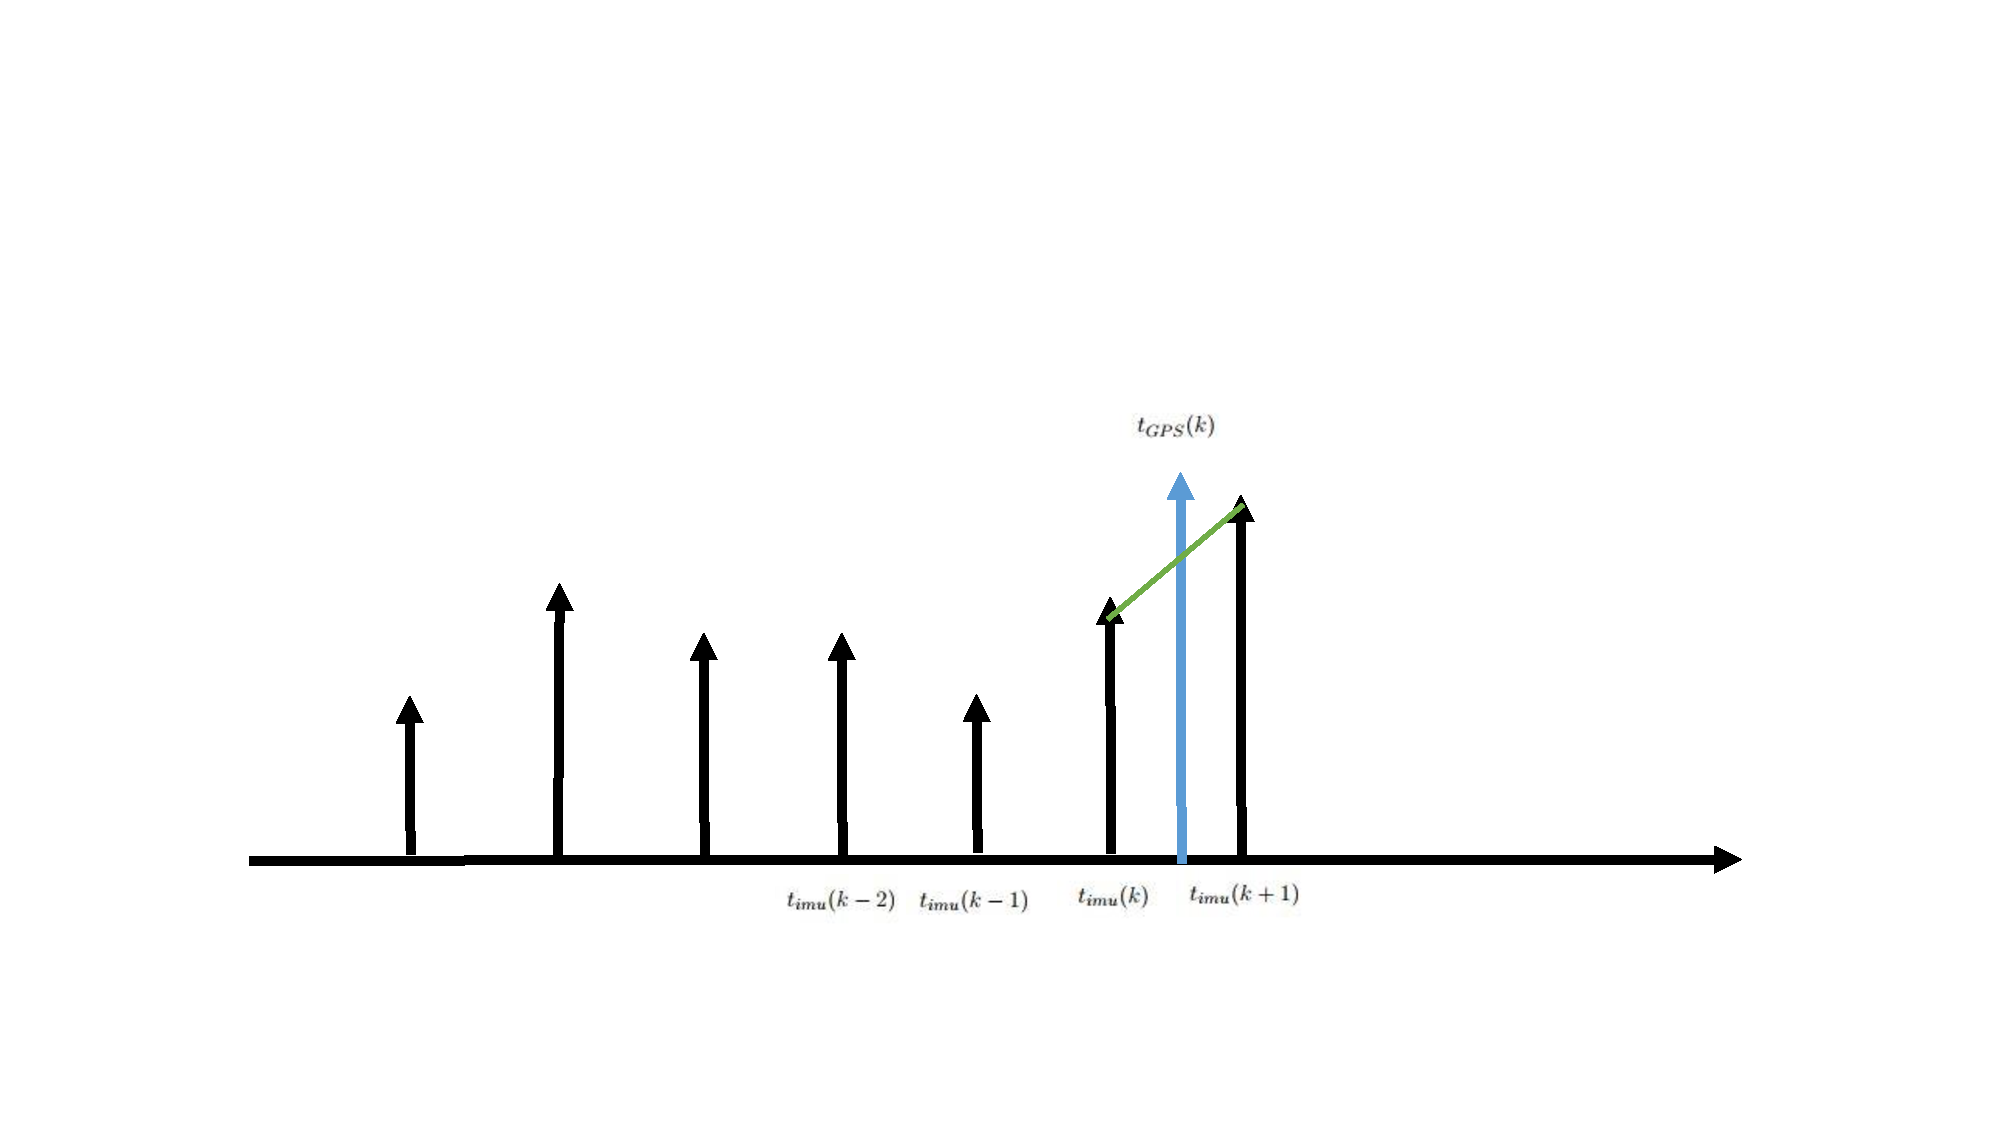
\includegraphics[width=0.8\textwidth]{Figures/linear.pdf}
\caption{Different update sequences \gls{imu} and \gls{gps}}
\label{Fig.different_update}
\end{figure}

The following linear interpolation equation is used for calculating the positions at $t_{GPS}(k)$
\begin{equation}
r_n(t_k(GPS) = r_n(t_{imu}(k)) + \frac{r_n(t_{imu}(k+1))-r_n(t_{imu}(k))}{t_{imu}(k+1)-t_{imu}(k)}(t_{GPS}(k)-t_{GPS}(k))
\end{equation}
 and the equations for the velocities 
 \begin{equation}
v_n(t_k(GPS) = v_n(t_{imu}(k)) + \frac{v_n(t_{imu}(k+1))-v_n(t_{imu}(k))}{t_{imu}(k+1)-t_{imu}(k)}(t_{GPS}(k)-t_{GPS}(k)).
\end{equation}
\subsection{Result}
The data provided by the Inertial Navigation System is working better than just using the raw \gls{gps} data, on some occasions. If the goal is to estimate the position, then it's better to use the \gls{ins} connected to a Kalman Filter, this can be seen in Fig. \ref{Fig:result_kalman}. As seen, the Filtered data is inaccurate in the beginning but after some time converges to the true value, true value as in the case of wanted value, and at some points even catches the wanted value. In comparison to the raw \gls{gps} data, the \gls{ins} is a better estimator for the user's position.
\begin{figure}[H]
\centering
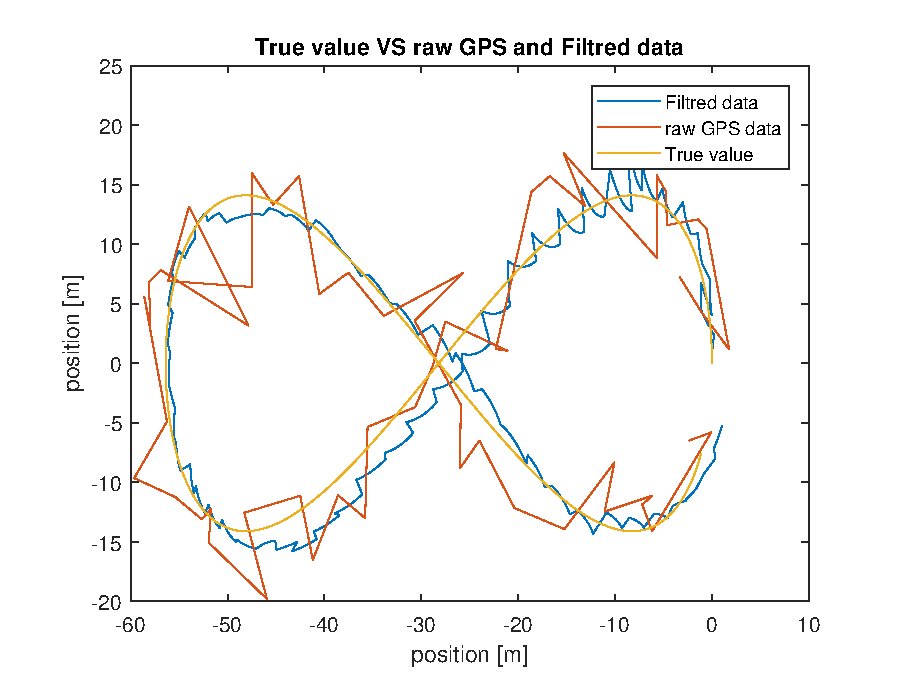
\includegraphics[width=0.5\textwidth]{result.eps}
\caption{True VS. Filtered and raw \gls{gps} data.}
\label{Fig:result_kalman}
\end{figure}



The Mean Squared Error, MSE for the position in XY plane, can be seen in Fig. \ref{Fig:mse} for both \gls{ins} and raw \gls{gps} data we can see that the error is lower for the \gls{ins} data, in both cases. 
\begin{figure}[H]
\centering
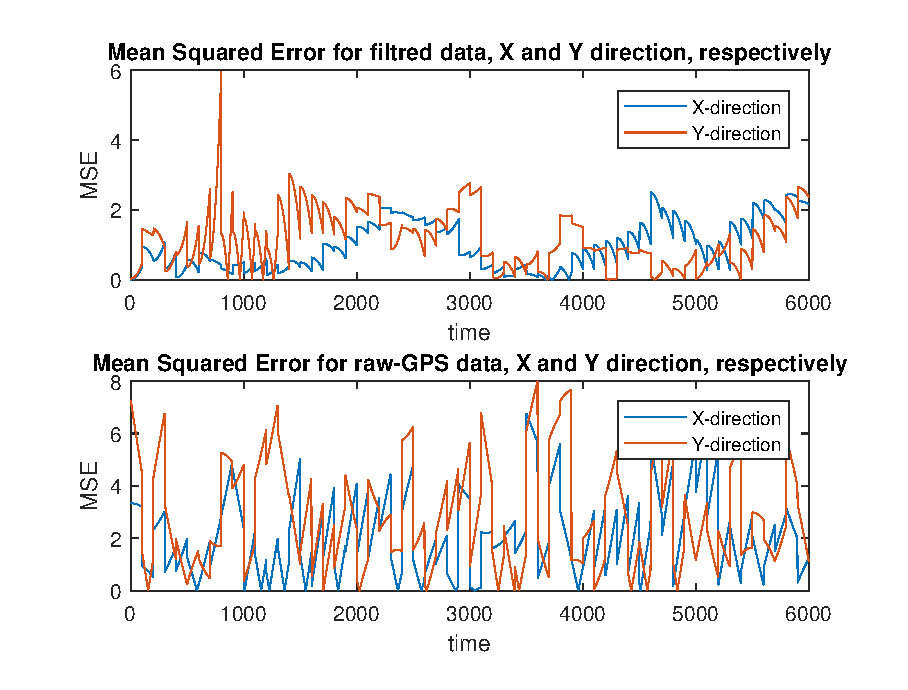
\includegraphics[width=0.5\textwidth]{mse.eps}
\caption{Mean Squared Error $XY$-plane separately.}
\label{Fig:mse}
\end{figure}

When estimating the height, i.e. $Z$-direction the result is poor for the \gls{ins}, the estimated value from the \gls{ins} is diverging from the true value, this can be seen in Fig. \ref{Fig:Height}. In this case, the \gls{gps} data is more accurate. 
\begin{figure}[H]
\centering
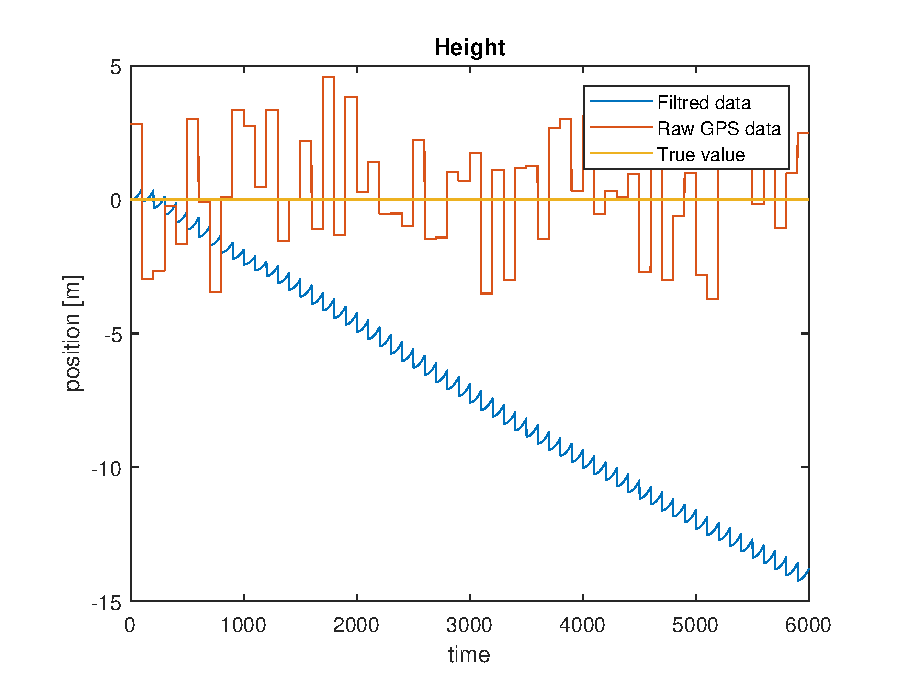
\includegraphics[width=0.5\textwidth]{Height.eps}
\caption{Height. True VS. Filtered and raw \gls{gps} data.}
\label{Fig:Height}
\end{figure}
The velocities in the $XY$ plane does not represent the true system in a good manner either this can be seen in Fig. \ref{Fig:velocity}. In this case, the \gls{gps} data is more accurate as well.

\begin{figure}[H]
\centering
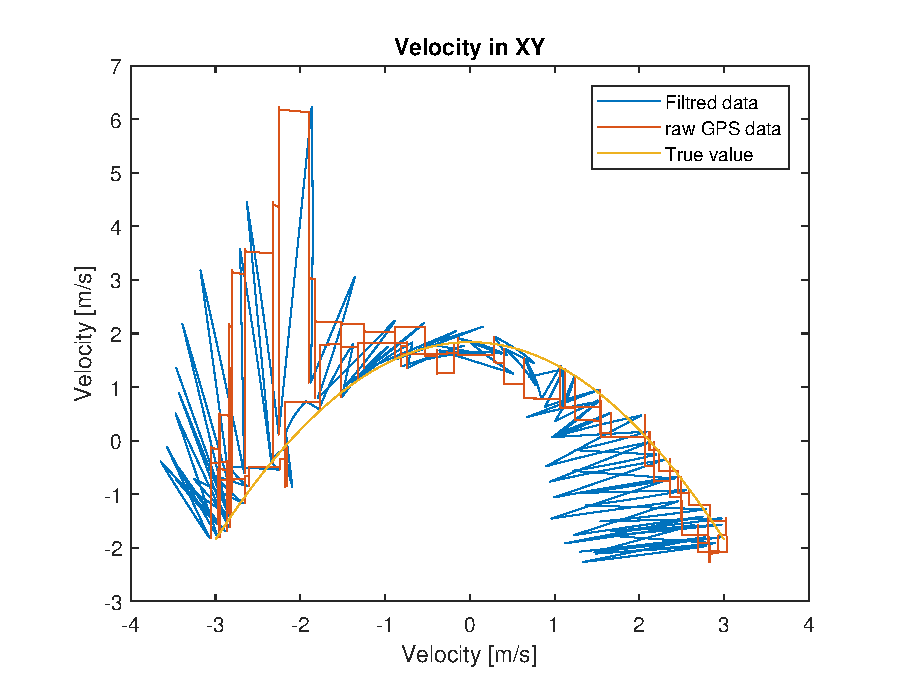
\includegraphics[width=0.5\textwidth]{velocity.eps}
\caption{The velocities in $XY$ plane.}
\label{Fig:velocity}
\end{figure}
\subsection{Discussion/Future Work}
Depending on what the user wants to measure, e.q. position in two dimensions, height or velocity, different sensors should be used. In the firts case, the \gls{ins} should be used in the case of the two latter the \gls{gps} should be used. \\

The Matlab code that exists, as right now, can read from the Nucleo Board using a serial read (assuming that the Nucleo Board uses the same firmware that was used by us), use stored data, (data created by our group) and also generate new data, with the \gls{imu} and \gls{gps} wanted characteristics. \\
Also, there is a static calibration program for the accelerometer. To see how the program works there exists a readme.txt file in the Matlab folder.\\

Implement a working real-time system for the sensor fusion between the \gls{gps} and \gls{ins}, there exits C-code for this already, but there is some serious bug/bugs which makes the error stored in $\hat{X}$ diverge exponentially. A serious attempt finding the problem was conducted and is narrowed down to a problem when calculating the Kalman Gain, $K_k$. Also, figure out why the height position diverges from the wanted value.\\

Improvements in the \gls{ins}/Kalman Filter implementation can be done as well, here are some thoughts that might be seen as guidelines/starting points to improve the system. \\
To obtain much more accurate information from the \gls{ins} one should consider more advanced techniques for calibrating the \gls{imu}. In this case, a static calibration technique was studied. This is done by keeping the \gls{imu} in a fixed position to observe the effect of gravity.
Consider implementing a more advanced technique, e.g. using this three-stage process.
\begin{itemize}
\item Coarse checking or evaluation using very simple test, such as a single stationary test on a bench, to establish the variance and standard deviation of the \gls{imu}, (gravity).
\item Static testing and studying the effects of natural phenomenon on the \gls{imu}.
\item Dynamic testing where the \gls{imu} is subjected to motions that should resemble the conditions out on the sea, e.g. constant waves hitting the sides of the boat. 
\end{itemize}
The purpose of this more advanced calibration technique is to determine the following parameters \cite{non-linear}
\begin{itemize}
\item scale factors
\item scale factor linearity
\item null bias error
\item axis alignment error, (might not be perfectly perpendicular)
\end{itemize}
Also, the dinghy's body may flex due to rough sea conditions, to solve this, implement one master \gls{ins} and one slave \gls{ins}, consider literature as Strap Down Inertial Navigation Technology, D.H. Titterton and J.L. Weston as a starting point for these different calibration methods. \newline 

A more advanced interpolation technique between \gls{imu} data and \gls{gps} data, here referencing to literature like Fundamentals of Scientific Computing, Bertil Gustafsson. E.g. Lagrange polynomial can be used to capture the true value better than using a linear interpolation.\newline


One should also try different types of control methods to see if one can achieve more accurate results or not, e.g. feed-forward method.\\
Weighted parameters if one believes the \gls{ins} more than the \gls{gps} or vice-versa, this question arises when e.g. the \gls{gps} is connected to many/few satellites or if the user is having a large/small velocity or sensor anomalies. \\ \\

